\chapter{\ifproject%
\ifcpe โครงสร้างและขั้นตอนการทำงาน\else Project Structure and Methodology\fi
\else%
\ifcpe โครงสร้างของโครงงาน\else Project Structure\fi
\fi
}

ในบทนี้จะกล่าวถึงหลักการ และการออกแบบระบบ

\makeatletter

% \renewcommand\section{\@startsection {section}{1}{\z@}%
%                                    {13.5ex \@plus -1ex \@minus -.2ex}%
%                                    {2.3ex \@plus.2ex}%
%                                    {\normalfont\large\bfseries}}

\makeatother
%\vspace{2ex}
% \titleformat{\section}{\normalfont\bfseries}{\thesection}{1em}{}
% \titlespacing*{\section}{0pt}{10ex}{0pt}

\section{Alice in Wonderland}

\begin{figure}
\begin{center}
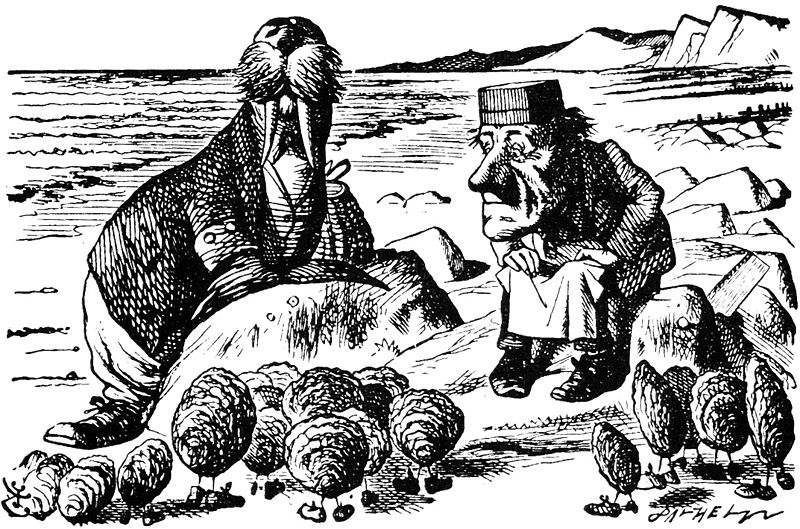
\includegraphics{800px-Briny_Beach.jpg}
\end{center}
\caption[Poem]{Check the exam schedule before enrolling.}
\label{fig:walrus}
\end{figure}

\begin{figure}
ท่านตรวจดูตารางสอบปลายภาคของแต่ละรายวิชาก่อนที่ท่านจะเลือกลงทะเบียนเรียนรายวิชานั้นหรือไม่
\begin{center}
\includegraphics{images/check_enrollment.png}\\[2ex]
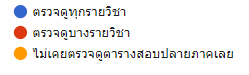
\includegraphics{images/type_check_enrollment.png}
\end{center}
\caption[Poem]{Check the exam schedule before enrolling.}
\label{fig:enroll}     
\end{figure}

\begin{figure}
\begin{center}
ท่านทราบหรือไม่ว่าสำนักทะเบียนมีวิธีการจัดตารางสอบปลายภาคอย่างไร
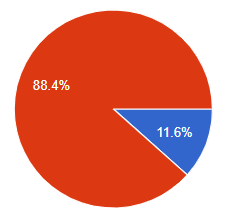
\includegraphics{images/redblue.png}\\[2ex]
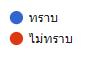
\includegraphics{images/type_redblue.png}
\end{center}
\caption[Poem]{Check the exam schedule before enrolling.}
\label{fig:enroll}     
\end{figure}

\begin{figure}
\begin{center}
ท่านทราบหรือไม่ว่าสำนักทะเบียนมีวิธีการจัดตารางสอบปลายภาคอย่างไร
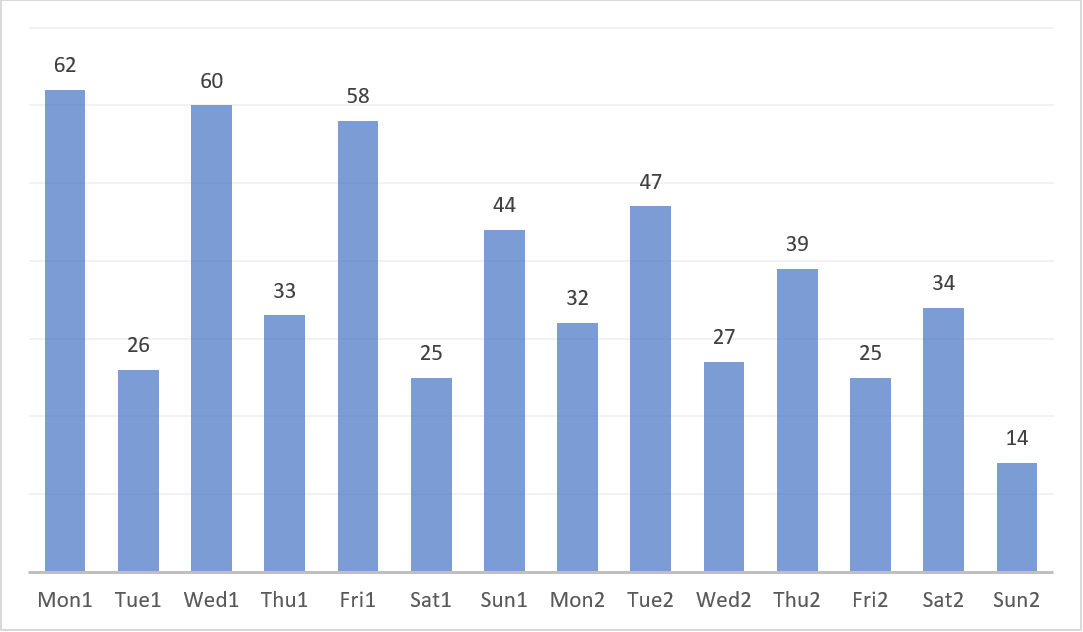
\includegraphics[width=\linewidth]{images/chart.png}
\end{center}
\caption[Poem]{Check the exam schedule before enrolling.}
\label{fig:enroll}     
\end{figure}
\begin{figure}
\begin{center}
ท่านทราบหรือไม่ว่าสำนักทะเบียนมีวิธีการจัดตารางสอบปลายภาคอย่างไร
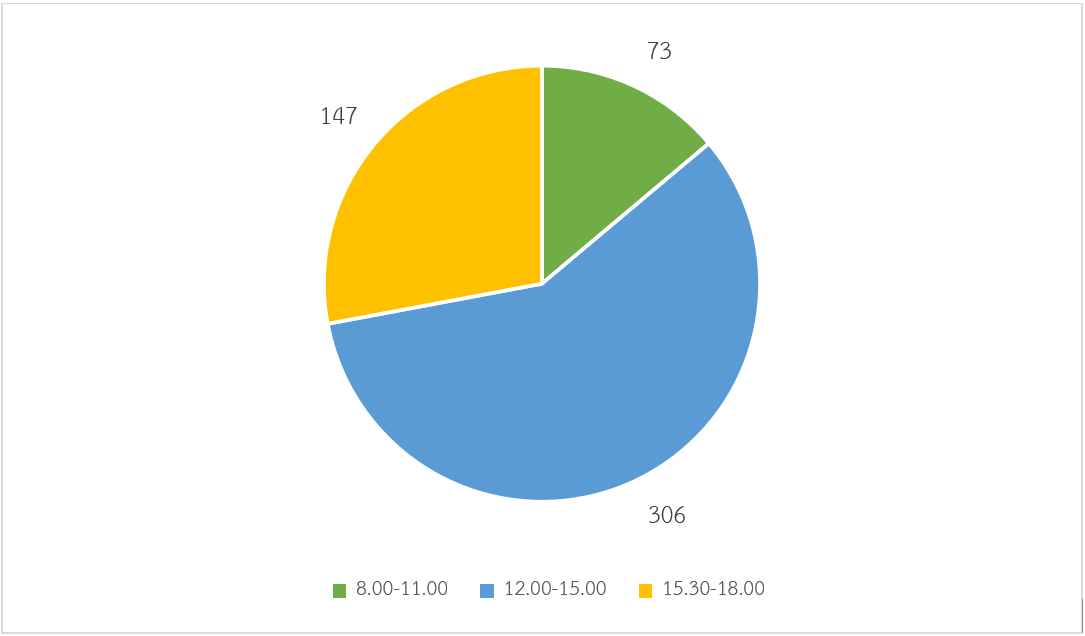
\includegraphics[width=\linewidth]{images/pie.png}
\end{center}
\caption[Poem]{Check the exam schedule before enrolling.}
\label{fig:enroll}     
\end{figure}
\begin{figure}
\begin{center}
ท่านทราบหรือไม่ว่าสำนักทะเบียนมีวิธีการจัดตารางสอบปลายภาคอย่างไร
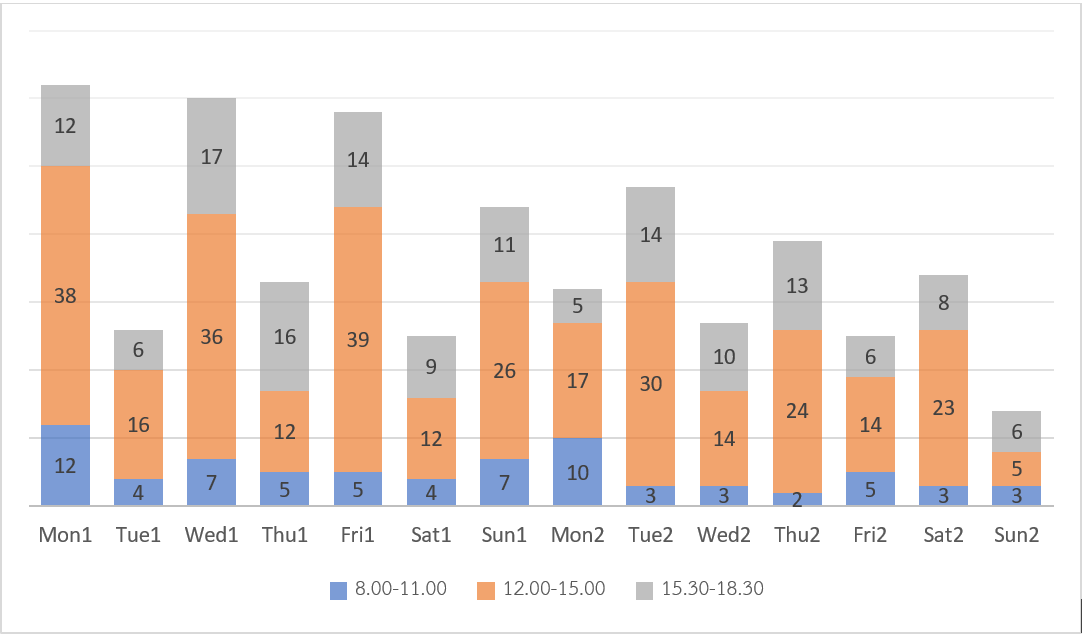
\includegraphics[width=\linewidth]{images/bar_chart.png}
\end{center}
\caption[Poem]{Check the exam schedule before enrolling.}
\label{fig:enroll}     
\end{figure}

\subsection{The Black Kitten}
  One thing was certain, that the WHITE kitten had had nothing to
do with it:---it was the black kitten's fault entirely~\cite{aiw}.  For the
white kitten had been having its face washed by the old cat for
the last quarter of an hour (and bearing it pretty well,
considering); so you see that it COULDN'T have had any hand in
the mischief.
\ref{fig:walrus}
  The way Dinah washed her children's faces was this:  first she
held the poor thing down by its ear with one paw, and then with
the other paw she rubbed its face all over, the wrong way,
beginning at the nose:  and just now, as I said, she was hard at
work on the white kitten, which was lying quite still and trying
to purr---no doubt feeling that it was all meant for its good.

  